\documentclass[tikz, border=10pt]{standalone}
% cf http://cloford.com/resources/colours/websafe1.htm
\definecolor{sv-all}{RGB}{255,153,255}
\definecolor{sv-gxe-m2}{RGB}{255,204,255}
\definecolor{sv}{RGB}{255,153,255}
\definecolor{m1}{RGB}{153,153,255}
\definecolor{m2}{RGB}{153,255,153}
\definecolor{ge}{RGB}{255,255,153}
\definecolor{sp}{RGB}{255,153,153}
\definecolor{vi}{RGB}{255,204,153}
\definecolor{ma}{RGB}{204,255,153}
\definecolor{hedo}{RGB}{153,153,255}
\definecolor{nap}{RGB}{153,255,153}

\usetikzlibrary{
  mindmap,
  decorations.pathreplacing,    % paths with shoapes of curly braces
  positioning,     % positions like above of node
  fit              % legend bounding box fitting all nodes
}
\tikzset{
  node distance=4ex and 4ex,
  % on grid,  % node distance from the centers
  every node/.style = {
    rectangle,
    minimum width=5em,
    minimum height=3ex,
    text depth=1pt,
    draw,
    outer sep = 2pt,
    inner sep = 3pt
  },
  every edge/.style = {->,draw},
  virtual/.append style = {draw=none, circle, minimum width=1em},
  % virtual/.append style = {draw, color=black!50},   % debugging purposes
  several-all/.append style = {fill = sv-all},
  several-gxe-m2/.append style = {fill = sv-gxe-m2},
  m1/.append style = {fill = m1},
  m2/.append style = {fill = m2},
  gxe/.append style = {fill = ge},
  sp/.append style = {fill = sp},
  vi/.append style = {fill = vi},
  ma/.append style = {fill = ma},
  aux/.append style = {fill = none},
  hedo/.append style = {fill = hedo},
  nap/.append style = {fill = nap},
  legendkey/.append style = {minimum width=3ex},
  legendtext/.append style = {draw=none, fill = black!10},
  ->,        % arrows for all
  >=stealth  % arrow type
}
\pgfdeclarelayer{background}
\pgfsetlayers{background,main}


\begin{document}

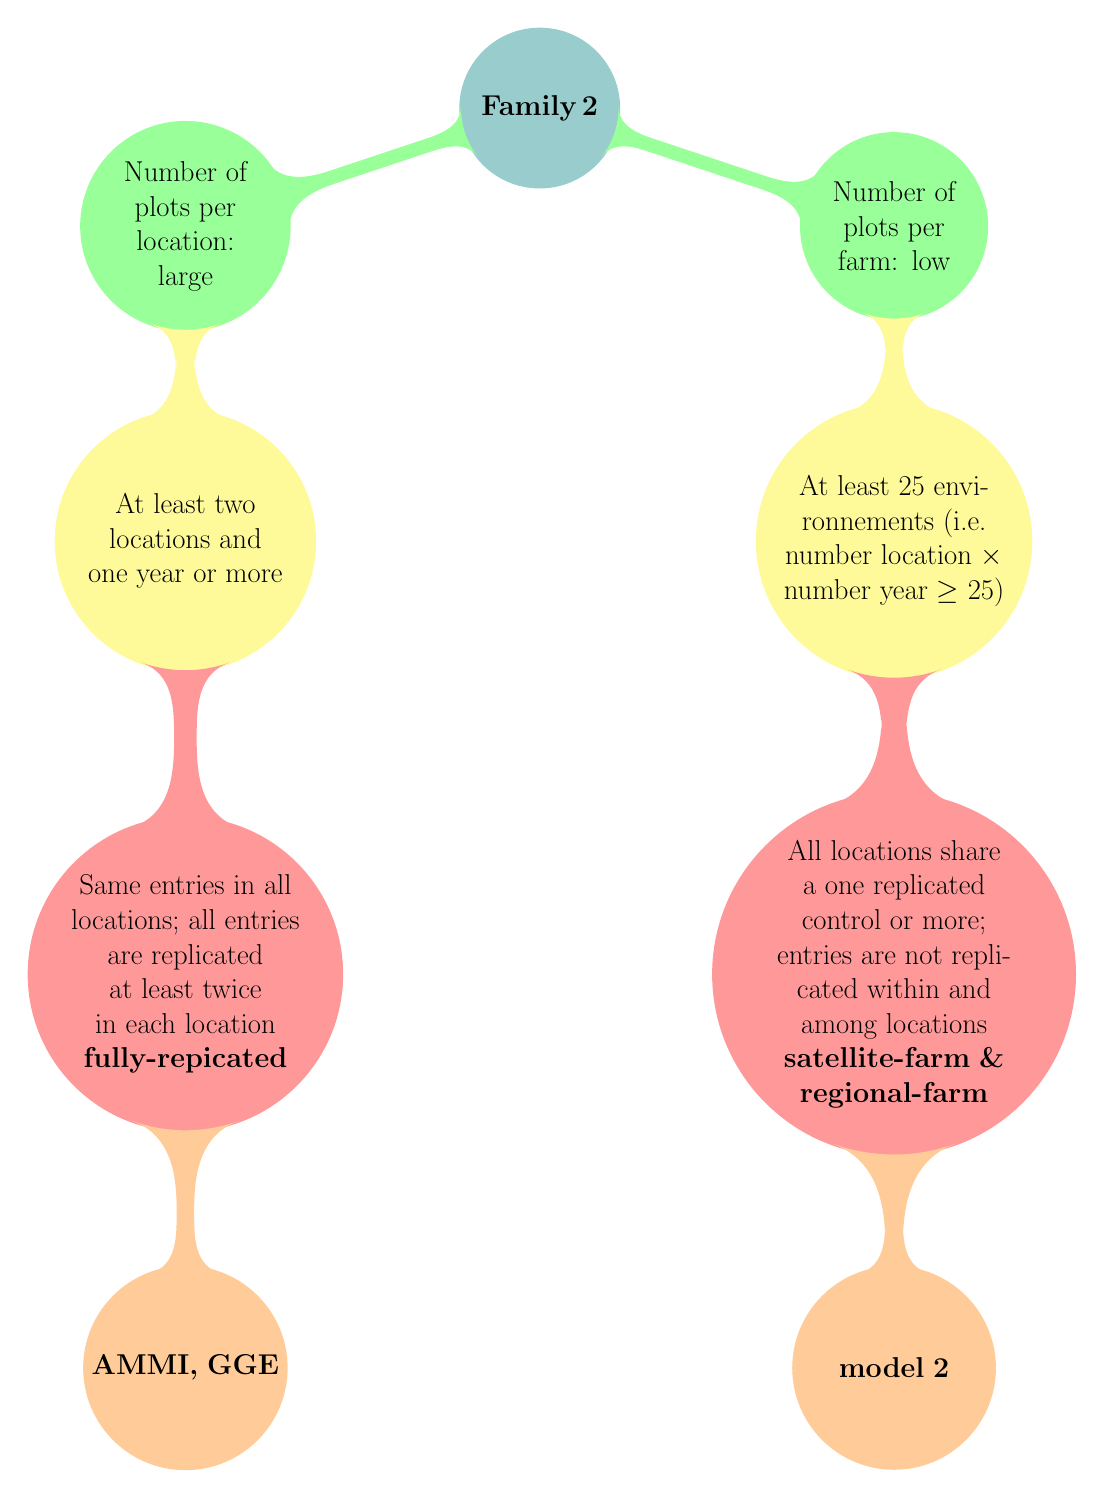
\begin{tikzpicture}[mindmap,
every node/.style=concept, concept color=teal!40,
every node/.append style={scale=0.5},
%every concept/.style={rectangle},
    level 1/.style={level distance=1.5cm, sibling distance= 9cm, concept color=green!40, font=\huge, text width=4cm},
    level 2/.style={level distance=4cm, sibling distance= 4cm, concept color=yellow!40, font=\huge, text width=6cm},
    level 3/.style={level distance=5.5cm, concept color=red!40, font=\huge, text width=6cm},
    level 4/.style={level distance=5cm, sibling distance= 3cm, concept color=orange!40, font=\huge, text width=5cm},
    ]

\node{\huge \textbf{Family 2} }
        child { node {Number of plots per location: large}
      		child { node {At least two locations and one year or more}
      			child { node {Same entries in all locations; all entries are replicated at least twice in each location \\ \textbf{fully-repicated} }
		      		child { node {\textbf{AMMI, GGE} }}
      			}
      		}
        }
        child { node {Number of plots per farm: low}
        	child { node {At least 25 environnements (i.e. number location $\times$ number year $\geq$~25)}
        		child { node { All locations share a one replicated control or more; entries are not replicated within and among locations \\ \textbf{satellite-farm \& regional-farm} }
					child { node {\textbf{model 2} }}
	        	}
        	}
        };
\end{tikzpicture}

\end{document}

